\documentclass{beamer}

\mode<presentation>{\usetheme{Madrid}}
\usepackage{graphicx}
\usepackage{multimedia}
\usepackage{hyperref}

\usepackage[utf8]{inputenc}
\usepackage[ngerman]{babel}
\usepackage{amsmath, amssymb, amsthm}

\usepackage{subcaption}
\usepackage[T1]{fontenc}
%\usepackage[sort&compress]{natbib}

\usepackage{lmodern}
\usepackage{caption}


\author[Jan Niclas Ruppenthal, Michael Feldmann, Philipp Geier]{}
\title[]{4. Übung zur Vorlesung
Virtual Reality\\ Serious Game}
\institute[Universität Trier]{}
\date[18. Juli 2024]{}
\beamertemplatenavigationsymbolsempty
\setbeamertemplate{footline}
{
  \leavevmode%
  \hbox{%
  \begin{beamercolorbox}[wd=.50\paperwidth,ht=2.25ex,dp=1ex,center]{author in head/foot}%
    \usebeamerfont{author in head/foot}\insertshortauthor%~~\beamer@ifempty{\insertshortinstitute}{}{(\insertshortinstitute)}
  \end{beamercolorbox}%
  \begin{beamercolorbox}[wd=.50\paperwidth,ht=2.25ex,dp=1ex,right]{date in head/foot}%
    \usebeamerfont{date in head/foot}\insertshortdate{}\hspace*{2em}
    \insertframenumber{} / \inserttotalframenumber\hspace*{2ex} 
  \end{beamercolorbox}}%
  \vskip0pt%
}
%—-------------------------------------------------------------

\begin{document}
{
  \usebackgroundtemplate{ 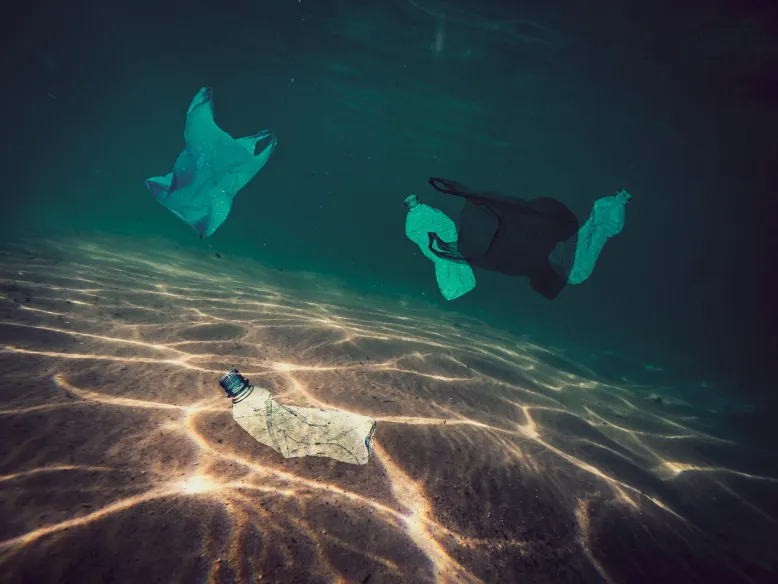
\includegraphics[width=\paperwidth]{img/plastic_bg}}
  \begin{frame}
    \maketitle
  \end{frame}
}
    
    %\begin{frame}
       % \frametitle{Inhalt}
		%\tableofcontents
	%\end{frame}
	
%—------------------------------------------------------

\begin{frame}{Thema}
\textbf{Müllsammeln im Korallenriff}
\begin{minipage}[c]{0.72\textwidth}
\begin{itemize}
\item Nachhaltigkeit
\item Förderung von Empathie
\item Bildung \& Aufklärung
\end{itemize}
\end{minipage}
\hfill
\begin{minipage}[c]{0.25\textwidth}
\begin{figure}
\centering

\includegraphics[width=0.9\textwidth, keepaspectratio]{img/waste}
\caption{\cite{a}}
\end{figure}
\end{minipage}
\end{frame}


\begin{frame}{Technischer Aufwand \& Qualität der technischen Umsetzung}
\begin{minipage}[c]{0.72\textwidth}
\begin{itemize}
\item Simulation von über 3000 Korallen
\item Unendliche Generierung der Landschaft
\item Simulation eines einfachen Schwarms
\end{itemize}
\end{minipage}
\hfill
\begin{minipage}[c]{0.25\textwidth}
\begin{figure}
\centering

\includegraphics[width=0.9\textwidth, keepaspectratio]{img/aufwand}
\caption{\cite{b}}
\end{figure}
\end{minipage}
\end{frame}

\begin{frame}{Authentizität \& Immersion der vermittelten Inhalte}
\begin{minipage}[c]{0.72\textwidth}
\begin{itemize}
\item Verschlechterung der Sicht
\item Korallensterben und Fischsterben
\item Simulation des Atems
\item Bewegung ist nur mithilfe des DPVs möglich
\item Faktenvideo am Ende des Spiels
\end{itemize}
\end{minipage}
\hfill
\begin{minipage}[c]{0.25\textwidth}
\begin{figure}
\centering

\includegraphics[width=0.9\textwidth, keepaspectratio]{img/immersion}
\caption{\cite{c}}
\end{figure}
\end{minipage}
\end{frame}

\begin{frame}{Nutzbarkeit \& Benutzererfahrung}
\begin{minipage}[c]{0.72\textwidth}
\begin{itemize}
\item Radar zur Müllortung
\item Rote Outline an den Müllobjekten
\item Bewegung: Steering durch Pointing-based und linearer Beschleunigung implementiert
\item Restart-Option
\end{itemize}
\end{minipage}
\hfill
\begin{minipage}[c]{0.25\textwidth}
\begin{figure}
\centering
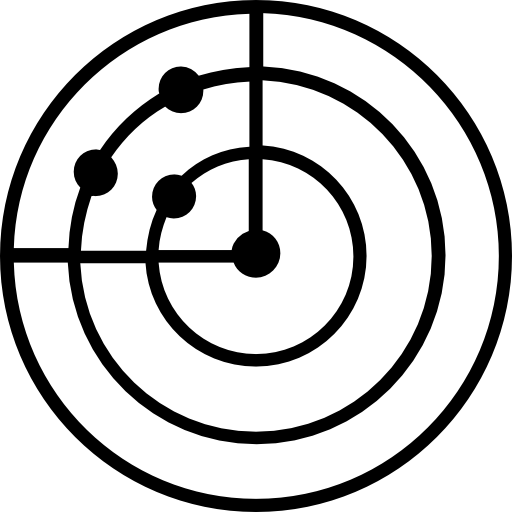
\includegraphics[width=0.9\textwidth, keepaspectratio]{img/radar}
\caption{\cite{d}}
\end{figure}
\end{minipage}
\end{frame}

\begin{frame}{Locomotion}
\textbf{Metapher}
\begin{itemize}
\item Pointing-based:\begin{itemize}
\item 3 DOF vTranslation
\item 0 DOF vRotation $\rightarrow$ nur physische Rotation möglich
\end{itemize}
\end{itemize}
\textbf{Travel-Task}
\begin{itemize}
\item Search
\end{itemize}
\end{frame}

\begin{frame}{Locomotion}
\textbf{Funktion}
\begin{itemize}
\item Maximalgeschwindigkeit: 5 Meter pro Sekunde
\end{itemize}
\begin{figure}
\centering
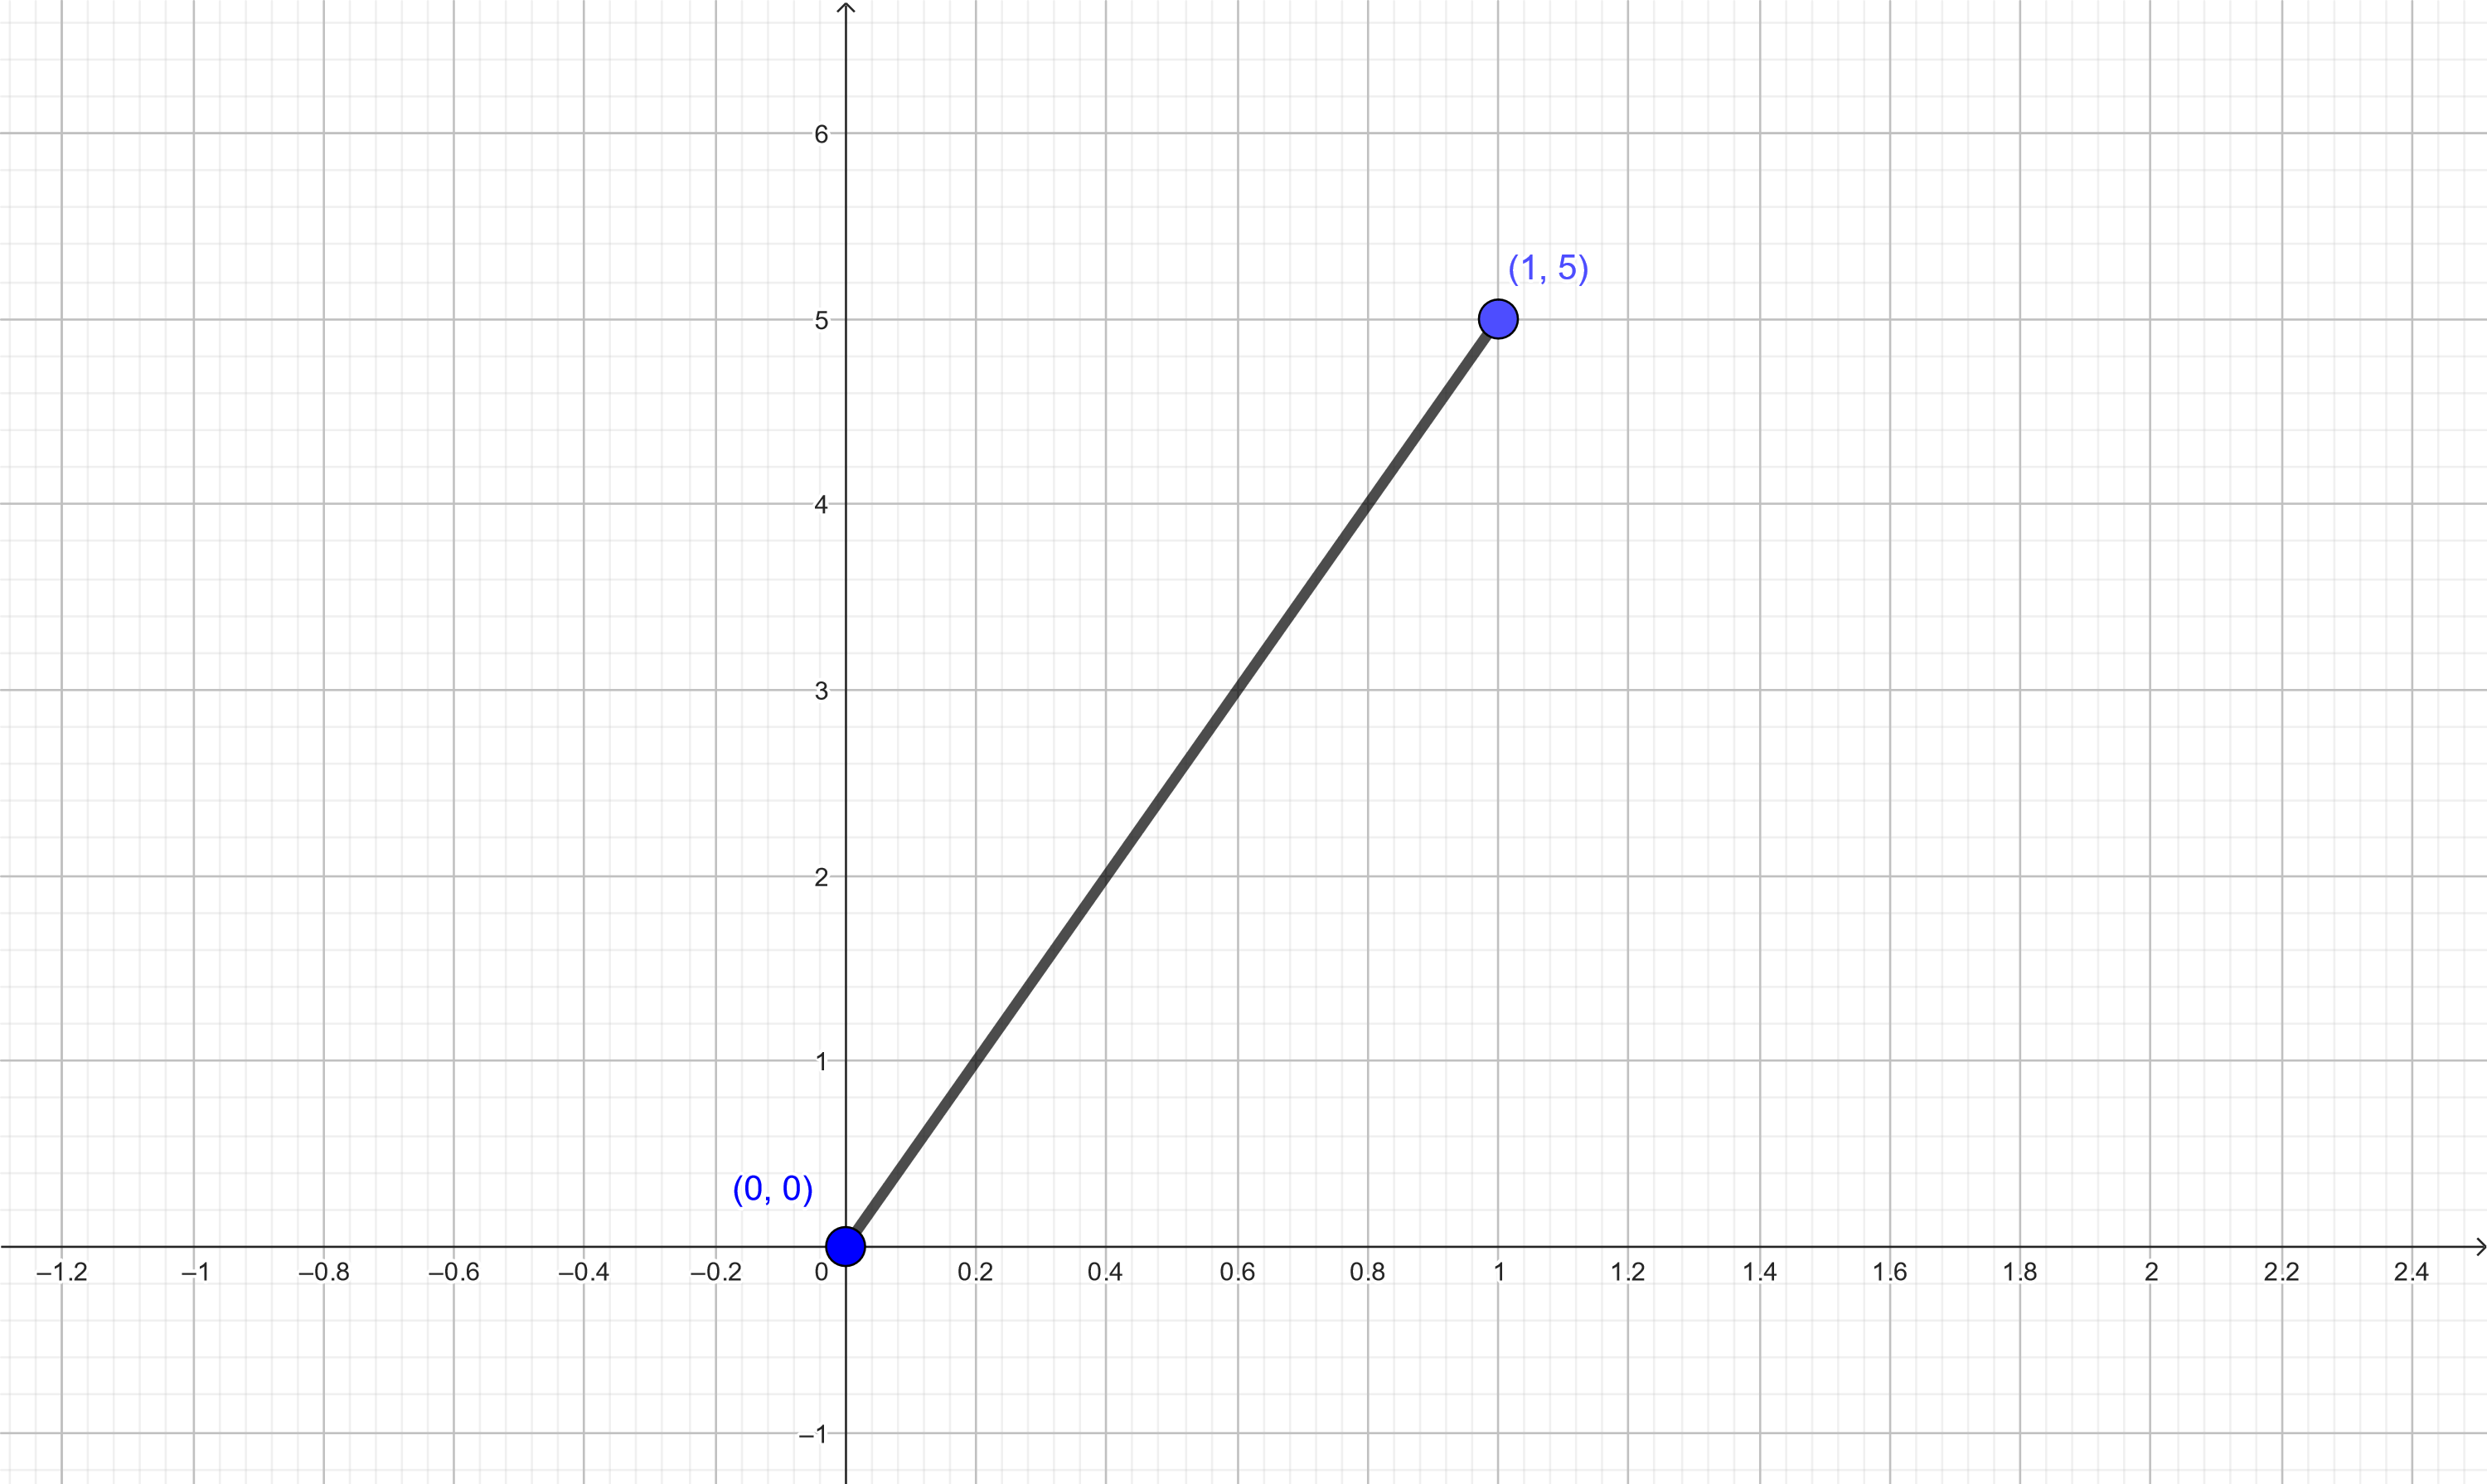
\includegraphics[width=.7\textwidth, keepaspectratio]{img/DPV}
\caption{Movement}
\end{figure}
\end{frame}

\begin{frame}{3D Interaktion \& multimodalem Feedback}
\begin{minipage}[c]{0.72\textwidth}
\begin{itemize}
\item Greifen des Mülls mithilfe eines Controllers
\item Vibration der Controller in Abhängigkeit der aktuellen Geschwindigkeit
\end{itemize}
\end{minipage}
\hfill
\begin{minipage}[c]{0.25\textwidth}
\begin{figure}
\centering

\includegraphics[width=0.9\textwidth, keepaspectratio]{img/cont}
\caption{\cite{e}}
\end{figure}
\end{minipage}
\end{frame}


\begin{frame}{Aufgabe}
\textbf{Ziel:} Möglichst viel Müll aufsammeln\\
\begin{minipage}[c]{0.49\textwidth}
\begin{figure}
\centering
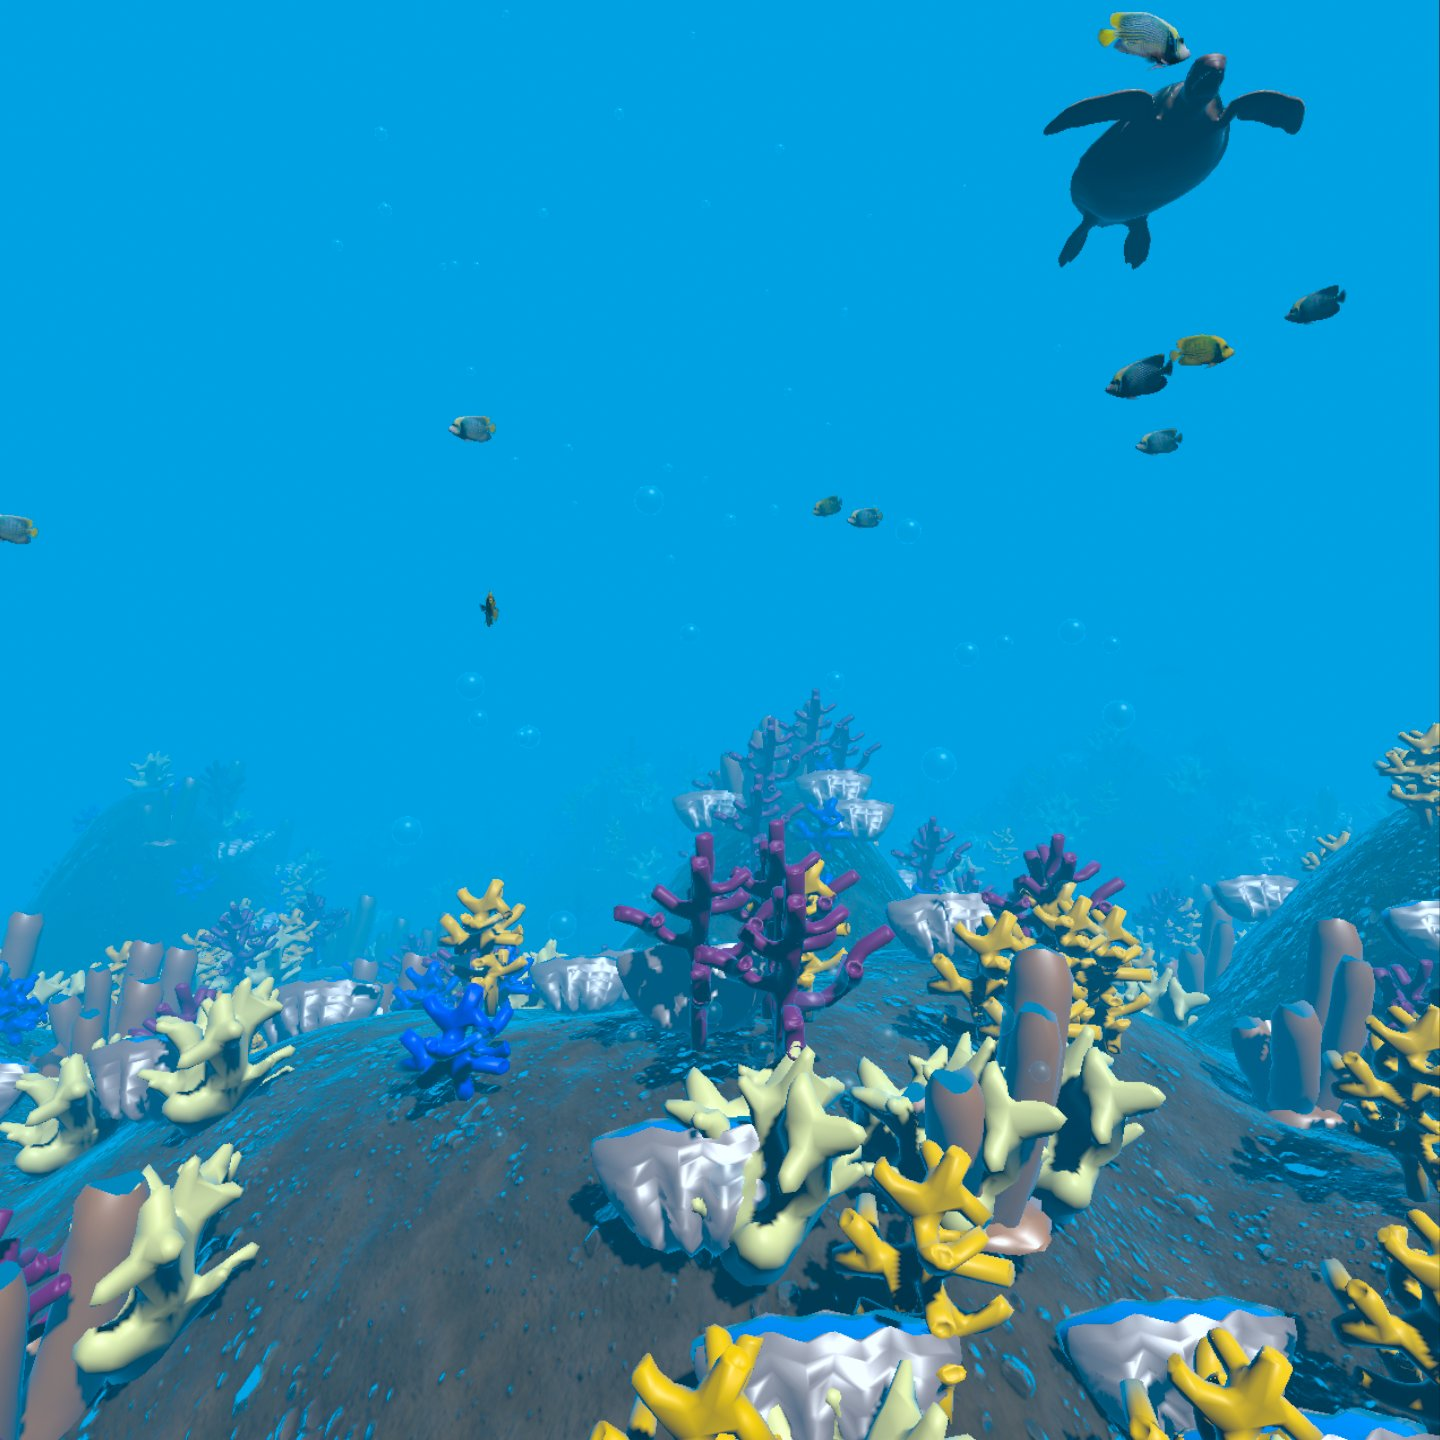
\includegraphics[width=\textwidth, keepaspectratio]{img/Vorher_Bild}
\caption{Vorher}
\end{figure}
\end{minipage}
\hfill
\begin{minipage}[c]{0.49\textwidth}
\begin{figure}
\centering
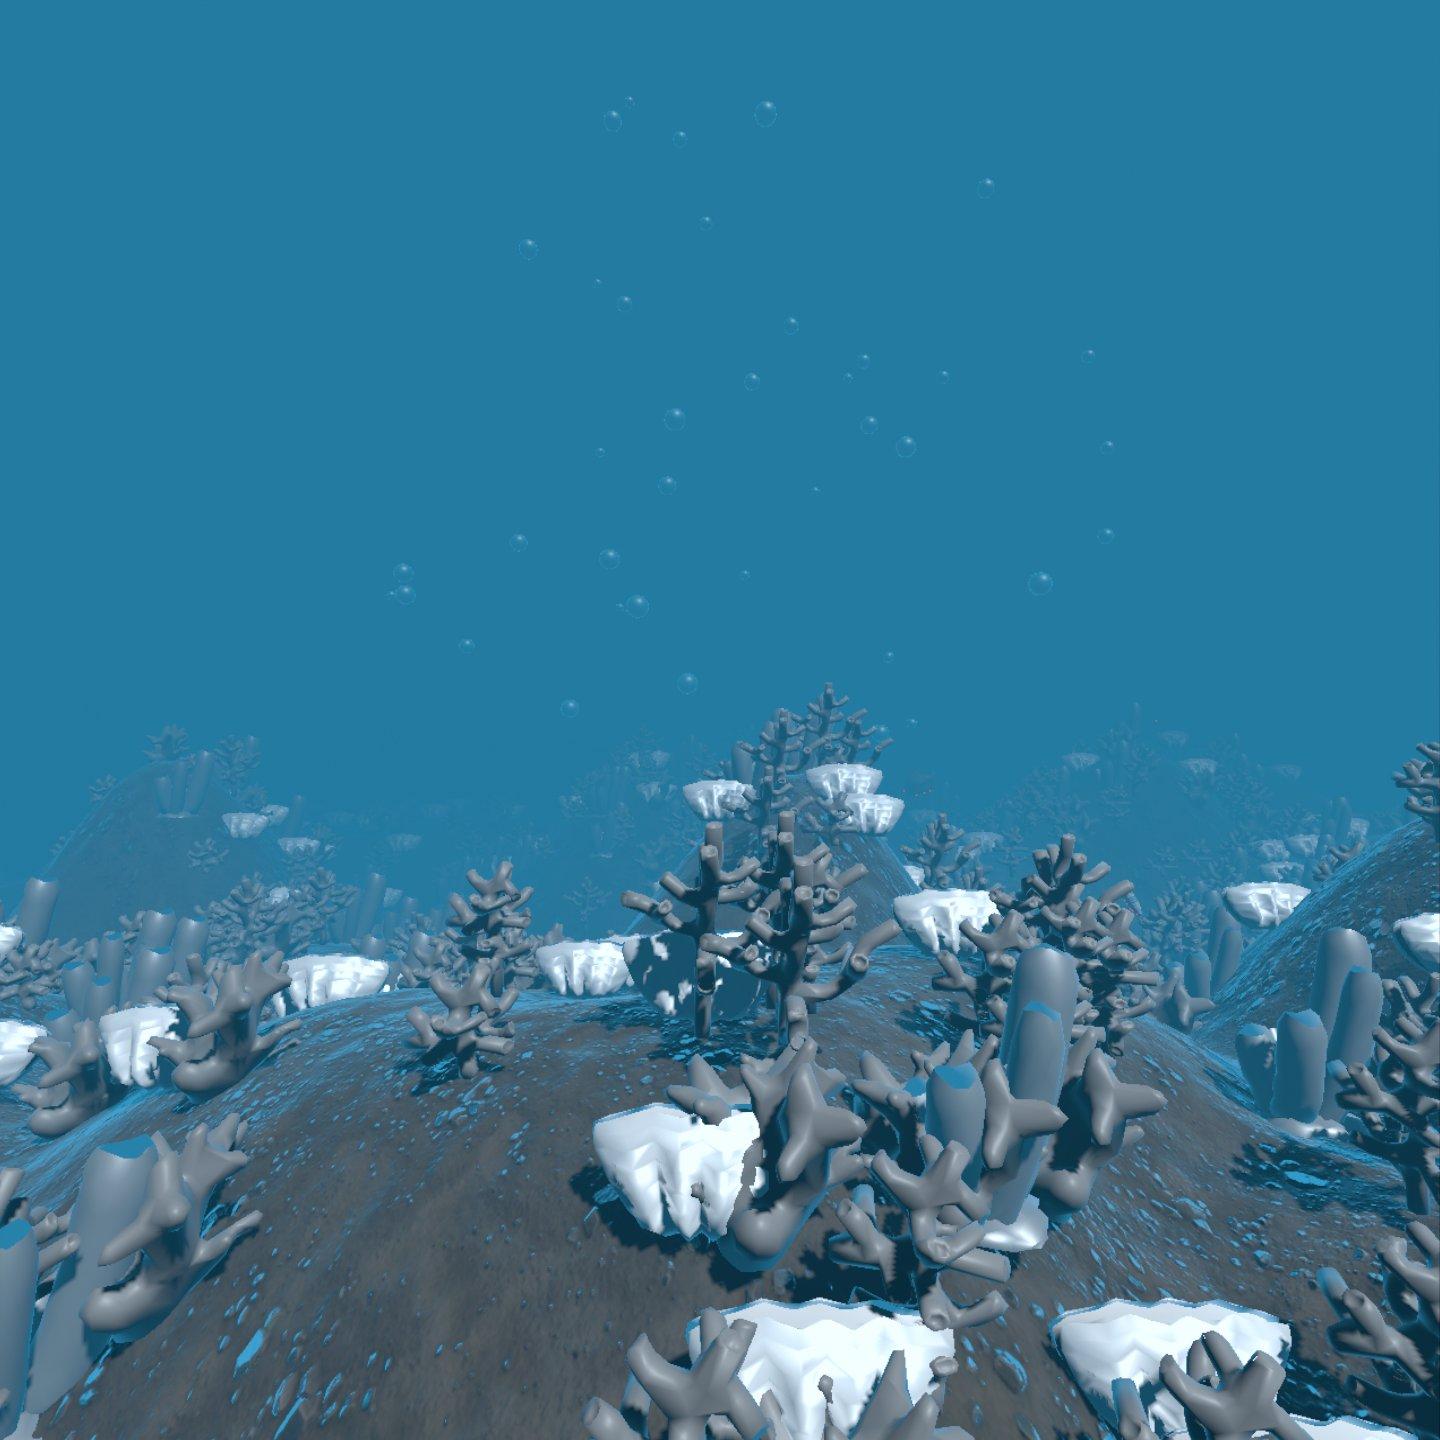
\includegraphics[width=\textwidth, keepaspectratio]{img/Nachher_Bild}
\caption{Nachher}
\end{figure}
\end{minipage}
\end{frame}


\begin{frame}{Gameplay}
\begin{figure}
    \centering
    \movie[externalviewer]{
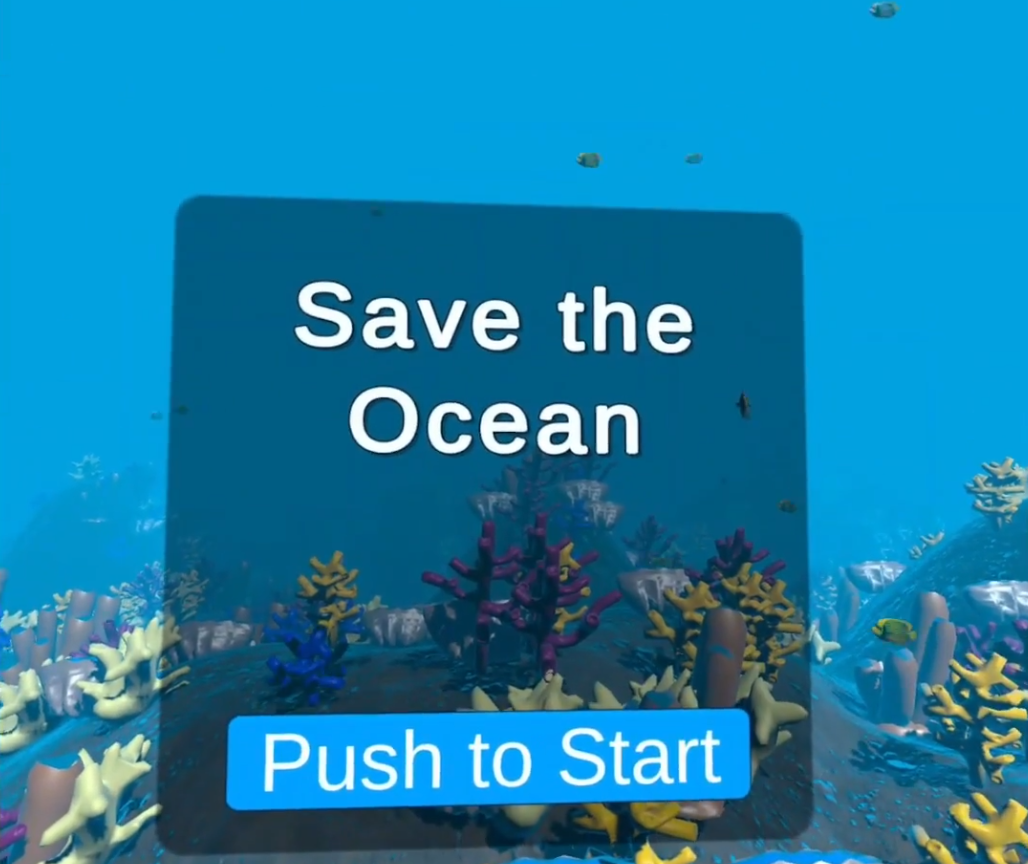
\includegraphics[width=0.6\textwidth, keepaspectratio]{img/video}
}{vid/SaveTheOcean_Presentation.mp4}
\caption{Gameplay}
\end{figure}
\end{frame}


\begin{frame}{Quellen}
	\begin{thebibliography}{1}
\bibitem{a}[1]{ https://cdn-icons-png.flaticon.com/512/535/535624.png }
\bibitem{b}[2]{ https://cdn-icons-png.flaticon.com/512/535/535624.png }
\bibitem{c}[3]{ https://static.thenounproject.com/png/981555-200.png }
\bibitem{d}[4]{ https://cdn-icons-png.flaticon.com/512/477/477840.png }
\bibitem{e}[5]{ https://static.thenounproject.com/png/4145521-200.png }
\bibitem{nick}[6]{ Assets: siehe README.txt}
\end{thebibliography}
\end{frame}


	
    	
    	
    	
\end{document}
